\documentclass[10pt]{article}
\usepackage[margin=0.95in]{geometry}
\usepackage[T1]{fontenc}
\usepackage{lmodern}
\usepackage{amsmath,amssymb}
\usepackage{booktabs}
\usepackage{graphicx}
\usepackage{caption}
\usepackage[hidelinks]{hyperref}
\usepackage{url}
\usepackage{microtype}
\captionsetup{font=small,labelfont=bf}
\setlength{\parskip}{3pt}
\emergencystretch=3em
\newcommand{\todo}[1]{\textbf{[TODO: #1]}}
\newcommand{\cn}{C_{\mathrm{norm}}}

\title{A Graph-Theoretic Mediation Layer for LLM Memory:\\Formalism, Audit, and Pre-Registered Evaluation}
\author{Krishna Sharma\\ \small MIT ADT University \todo{confirm affiliation and add contact e-mail}}
\date{Draft of 3 November 2026 (IST)}

\begin{document}
\maketitle

\begin{abstract}
We study a ``Sandwich'' memory architecture for LLM assistants: a primary model drafts an answer, a graph memory over past conversation turns mediates retrieval, and a secondary model refines the answer. The original specification of the graph layer was informal and, on audit, contained undefined, unbounded and internally contradictory quantities. We (i) give a bounded, fully specified version (theory v1.1), listing every audit fix; (ii) evaluate it with experiments whose hypotheses, predictions, falsifiers and metrics were committed to version control before each run, using paired bootstrap, sign-flip tests and Holm correction; and (iii) report the results as they came out, including the negative ones. On LoCoMo (1{,}536 questions) reciprocal rank fusion of BM25 and dense retrieval is a strong baseline (all-evidence@10 $0.493$ versus $0.391$ for dense retrieval alone). On the 277 multi-hop questions that need several evidence turns, the graph layer does not meet the pre-registered bar of $+0.03$ over fusion: the dev-selected configuration changes nothing ($0.000$, CI $[0.000,0.000]$), a more aggressive configuration gains $+0.018$ ($[-0.004,+0.043]$), and association weights, shuffled weights and ablated factors are indistinguishable. With a 1.5B reader, graph context and fusion context give the same answer F1 ($-0.001$, $[-0.015,+0.013]$). We find no evidence of benefit from the weighting formula and weak evidence that graph topology beats random edges. The contribution is the formalism, the audit, the evaluation protocol with its logged dead ends, and a reproducible negative result. All experiments are CPU-only with small models and no LLM judge; they do not settle what larger readers would do.
\end{abstract}

\section{Introduction}
Chat assistants that persist over many sessions need a memory that decides which past turns to show the model. Common designs score turns by relevance, recency and importance \cite{park2023generative}, manage tiers of memory \cite{packer2023memgpt}, or spread activation over a graph built from the text \cite{gutierrez2024hipporag}. A related line has a model critique and revise its own output \cite{madaan2023selfrefine}.

This paper examines one combination of these ideas, the \emph{Sandwich} design: draft (primary LLM) $\rightarrow$ graph memory $\rightarrow$ refine (secondary LLM). The design started as a loosely specified ``consciousness layer'' motivated by an informal analogy to integrated-information theory \cite{tononi2008iit}; that analogy is not used again here, makes no claim about machine consciousness, and no quantity below is anything other than an engineering quantity on a graph. What remains is an architecture and an evaluation question: \emph{does a weighted association graph between two LLM calls improve retrieval or answers over a strong retrieval baseline?}

We make three contributions. (1) A bounded, fully specified formalism (Section~\ref{sec:formalism}) obtained by auditing the original equations; the audit found 20 issues, each fix tagged by whether it is mathematically required or an arbitrary default. (2) A pre-registered evaluation protocol (Section~\ref{sec:protocol}) in which hypothesis, numeric prediction, falsifier, primary metric and configuration are committed before the run, and the run logger refuses to start on a dirty source tree. (3) The results (Section~\ref{sec:results}), which are mostly negative: the graph layer's headline hypothesis was falsified on LoCoMo multi-hop retrieval and end-to-end QA, and the weighting formula carries no demonstrable information.

\section{Related Work}
\textbf{Retrieval-augmented generation} conditions a generator on retrieved passages \cite{lewis2020rag}. Our baselines are BM25 \cite{robertson2009bm25}, a dense MiniLM bi-encoder \cite{wang2020minilm,reimers2019sbert}, and their reciprocal rank fusion \cite{cormack2009rrf}. \textbf{Agent memory.} Generative Agents retrieve from a memory stream by a sum of recency, importance and relevance \cite{park2023generative}; MemGPT manages a hierarchy of context tiers \cite{packer2023memgpt}. Our $T$ (time decay) factor is a recency term of the first kind, but we study it as a weight on graph edges rather than a score on nodes. \textbf{Graph retrieval.} HippoRAG runs personalised PageRank \cite{page1999pagerank} over a knowledge graph of extracted entities to retrieve passages \cite{gutierrez2024hipporag}. Our retrieval step is the same operator over a graph of conversation turns whose edges come from embedding similarity; we do not extract entities, so our results say nothing about HippoRAG itself. \textbf{Refinement.} Self-Refine iterates feedback and revision with one model \cite{madaan2023selfrefine}; the Sandwich's secondary pass is a single refinement that is additionally given retrieved memory. \textbf{Benchmarks.} LongMemEval tests long-term interactive memory of chat assistants \cite{wu2025longmemeval}; LoCoMo provides very long multi-session conversations with question categories including multi-hop and temporal questions \cite{maharana2024locomo}. We use LongMemEval-S for development and LoCoMo for the pre-registered confirmatory runs.

\section{Formalism: the Sandwich Model, theory v1.1}\label{sec:formalism}
\textbf{Pipeline.} For a user query $q$ and history turns $x_1..x_N$: the primary model produces a draft $d=f_1(q,\text{recent window})$; the graph layer returns memories $M=\mathcal G(q)$; the secondary model returns $a=f_2(q,M)$, optionally also given $d$. Each turn is a node with a unit embedding $v_i\in\mathbb R^{384}$ (MiniLM-L6-v2), a formation time $t_i$ and a lexicon-based valence $e_i\in[-1,1]$.

\textbf{Edge weight.} With half-life $h$ and valence factor $F$,
\begin{align}
S_{ij}&=\max(0,\cos(v_i,v_j)), \quad T_{ij}=\exp(-\ln 2\,|t_i-t_j|/h), \quad F_{ij}=1+\kappa_E\tfrac{|e_i|+|e_j|}{2},\\
W_{ij}&=\frac{S_{ij}\,T_{ij}\,F_{ij}\,R_{ij}}{W_{\max}}\in[0,1],\qquad W_{\max}=(1+\kappa_E)R_{\max}.
\end{align}
Ablated factors are set to 1 and dropped from $W_{\max}$. $R_{ij}\in[1,R_{\max}]$ is a bounded, saturating reinforcement updated only on traversed edges; without learning $R\equiv1$. Edges exist for the top $k_e=8$ neighbours of each node by $\tau_{ij}=\alpha e_{ij}b+\beta S_{ij}+\rho\tilde R_{ij}>\theta$ ($\theta=0.2$), symmetrised. With mood $b=0$ and $R\equiv 1$, the topology is a thresholded cosine $k$NN graph.

\textbf{Activation.} $P_{ij}=W_{ij}/\sum_k W_{ik}$ (self-loop for empty rows). The cue $I$ is the query's cosine scores restricted to the top $m=5$ nodes and normalised to the simplex. Activation iterates
\begin{equation}
A^{(t+1)}=\zeta P^\top A^{(t)}+(1-\zeta)I,\qquad A^{(0)}=I,
\end{equation}
whose unique fixed point $A^\star$ is personalised PageRank of $I$. Coherence is $\cn=A^\top W A/(\sum_i A_i)^2\in[0,1]$. A path from the best cue match to $\arg\max A^\star$ is found by A$^*$ \cite{hart1968astar} with edge cost $-\log W_{ij}$ and a scaled admissible heuristic. Retrieved memories are the goal node, the path, then nodes in decreasing $A^\star$ order.

\textbf{Re-ranking form.} For a first-stage score $s$ (e.g.\ RRF), the graph acts as a bonus: $\mathrm{score}_i=(1-w)\,\mathrm{mm}(s_i)+w\,\mathrm{mm}(A^\star_i)$ with min-max scaling $\mathrm{mm}$ and $A^\star$ seeded by the first stage's top 5. We use two settings: \emph{S-only} ($w=0.1$, $\zeta=0.5$, $W=S$; chosen on a development half of LongMemEval-S) and \emph{strong} (full $W$, $w=0.5$, $\zeta=0.85$).

\textbf{Audit fixes (v1.0$\to$v1.1).} The audit (20 items) found, among others: no input $I$ or update rule for activation was given; the refine trigger $\lambda$ was stated in contradictory directions; $C$ and $R$ were unbounded; ``success'' and the A$^*$ heuristic were undefined (the latter could be inadmissible); $1+E_{ij}$ can be $\le 0$; $W$ was unnormalised; symmetric factors were placed on a directed graph; the secondary model ``updating $W$'' was over-determined. Each fix is tagged mathematically required or arbitrary in the specification. Two further corrections came from experiments: (a) the claim that rescaling $R$ does not change anything holds for $P$ and $A$ but not for A$^*$ paths, because $-\log$ adds a per-hop penalty $\log W_{\max}$ (11 of 470 paths changed); (b) $\cn$ is normalised by the theoretical maximum, so its scale depends on which factors are active and it is comparable only within one configuration. The design did not change after the LoCoMo runs, so the current version remains v1.1.

\section{Experimental Protocol}\label{sec:protocol}
\textbf{Pre-registration.} For every run we wrote, and committed to git before the run, the hypothesis, a numeric or directional prediction, a falsifier, the primary metric and its label, the configuration and the seed. Our run logger refuses to start if source, experiment or test files are uncommitted and stores the commit hash, package versions and wall-clock time with each result. This is a self-registration with commit timestamps, not a third-party registry. Dead ends are logged (one aborted attempt is described below).

\textbf{Data.} LoCoMo (10 conversations, 5{,}882 turns, 1{,}986 questions, CC BY-NC 4.0) \cite{maharana2024locomo}. Questions in categories 1--4 (multi-hop, temporal, open-domain, single-hop) with at least one valid evidence turn form the full population ($N=1{,}536$); category 5 (adversarial) is excluded. Evidence identifiers were cleaned by regular expression; 4 questions lost one or more identifiers. The \emph{primary multi-hop population} is category 1 with at least two valid evidence turns ($N=277$). No text exceeds the 256-word-piece limit of the encoder.

\textbf{Metric.} \emph{All-evidence@$k$} is $1$ if every valid evidence turn is in the top-$k$ retrieved turns. We also report evidence recall (fraction@$k$) and any-evidence@$k$ as secondary, undecisive metrics. For QA we use the official LoCoMo partial token-F1 for category 1 (re-implemented, because the official script imports packages we do not use); there is no LLM judge and no paid API.

\textbf{Statistics.} Percentile bootstrap over questions ($B=10^4$, seed 0) for CIs; paired two-sided sign-flip test ($B=2\times10^4$); Holm correction~\cite{holm1979} within each pre-registered family. Conversation-clustered sensitivity analyses are reported where they matter. Secondary metrics are not corrected for multiplicity and are labelled descriptive.

\textbf{Runs.} R-2026-11-03-02 (confirmatory): H1, RRF(BM25, cosine; $k{=}60$) beats cosine and BM25 on all-evidence@10 ($N{=}1536$). R-2026-11-03-03: H2, on the primary multi-hop population the graph re-ranker beats RRF by $\ge0.03$ on all-evidence@10; \emph{falsified if} the CI upper bound of (S-only $-$ RRF) is below $0.03$ or S-only does not beat shuffled-$W$. It includes shuffled-$W$ (3 seeds), random-edge and random-weight controls, and S/T/E/R/A$^*$ ablations (20 paired tests in the Holm family). R-2026-11-03-04: QA with Qwen2.5-1.5B-Instruct \cite{qwen2024qwen25} (bf16, CPU, greedy, 10 turns of context in chronological order): arms Z closed-book, A RRF context, B graph-bonus context, C Sandwich retrieval (graph as first stage) without draft, D as C with the closed-book draft in the prompt. Primary label B$-$A; falsifier: CI upper bound of B$-$A below $+0.02$.

\textbf{Deviation.} A first attempt of R-03 was aborted because of BLAS thread oversubscription (numpy was imported before thread caps were set). No result had been seen; the fix touched no retriever, metric, configuration or statistic, and the same run id was re-run. The aborted directory is kept.

\textbf{Caveat on development data.} The re-ranker settings were chosen on a development half of LongMemEval-S and transferred unchanged to LoCoMo. LoCoMo was not used to tune anything.

\section{Results}\label{sec:results}
\subsection{Fusion baseline (R-2026-11-03-02)}
\begin{table}[h]
\centering\small
\begin{tabular}{lcc}\toprule
 & All cat.\ 1--4 ($N{=}1536$) & Multi-hop primary ($N{=}277$)\\\midrule
BM25 & 0.467 [0.443, 0.492] & 0.058 [0.032, 0.087]  \\
Cosine (MiniLM) & 0.391 [0.367, 0.415] & 0.079 [0.051, 0.112]  \\
RRF & 0.493 [0.469, 0.518] & 0.105 [0.072, 0.141]  \\
RRF $-$ cosine (paired) & +0.102 [+0.081, +0.124] & +0.025 [-0.007, +0.061]  \\
RRF $-$ BM25 (paired) & +0.026 [+0.007, +0.045] & +0.047 [+0.014, +0.079] 
\\\bottomrule
\end{tabular}
\caption{All-evidence@10, mean [95\% bootstrap CI]. RRF--BM25 on all categories has Holm $p=0.010$; clustered by conversation it is $+0.027$ [$-0.006,+0.063$], better in 7 of 10 conversations. RRF--cosine is better in 10 of 10.}\label{tab:rrf}
\end{table}
H1 was confirmed under the pre-registered rule (both Holm $p<0.05$): RRF--cosine $+0.102$, which is larger than predicted ($[+0.02,+0.08]$), and RRF--BM25 $+0.026$, inside the prediction. On the multi-hop primary population the three retrievers are low (RRF $0.105$); RRF--cosine is not distinguishable from zero and RRF--BM25 has Holm $p=0.13$ in the 20-test family of R-03. Overall, the fusion advantage is robust against the dense retriever and fragile against BM25.

\subsection{Graph versus fusion on multi-hop retrieval (R-2026-11-03-03)}
\begin{table}[h]
\centering\small
\begin{tabular}{lccc}\toprule
Retriever & All-evidence@10 & Diff.\ vs RRF & $p_{\mathrm{Holm}}$\\\midrule
RRF baseline & 0.105 [0.072, 0.141] & -- & --\\
RRF + S-only graph bonus & 0.105 [0.072, 0.141] & +0.000 [+0.000, +0.000] & --  \\
RRF + full-$W$ graph bonus (strong) & 0.123 [0.087, 0.162] & +0.018 [-0.004, +0.043] & 1.00  \\
Graph as first stage (v1) & 0.079 [0.051, 0.112] & -0.025 [-0.058, +0.007] & 1.00 
\\\bottomrule
\end{tabular}
\caption{Primary multi-hop population ($N=277$). The S-only row is the pre-registered primary comparison; its CI is degenerate because the all-evidence outcome is identical on all 277 questions (raw $p=1.0$). Holm is over the 20-test exploratory family.}\label{tab:graph}
\end{table}
\textbf{H2 was falsified} (both falsifiers fired). The S-only re-ranker changes the 10-turn set for only 5 of 277 questions (by evidence recall) and never flips the all-evidence outcome. The strong configuration gains $+0.018$ with a CI that includes zero and has an upper bound ($+0.043$) above the margin, so we cannot rule out a small gain from \emph{that} configuration; but it was not the pre-registered primary and is not significant. Using the graph as the first stage is worse than RRF in point estimate ($-0.025$, CI includes 0) and equal to cosine. Nothing in the 20-test family survives Holm (smallest $p_{\mathrm{Holm}}=0.13$).

\begin{figure}[h]
\centering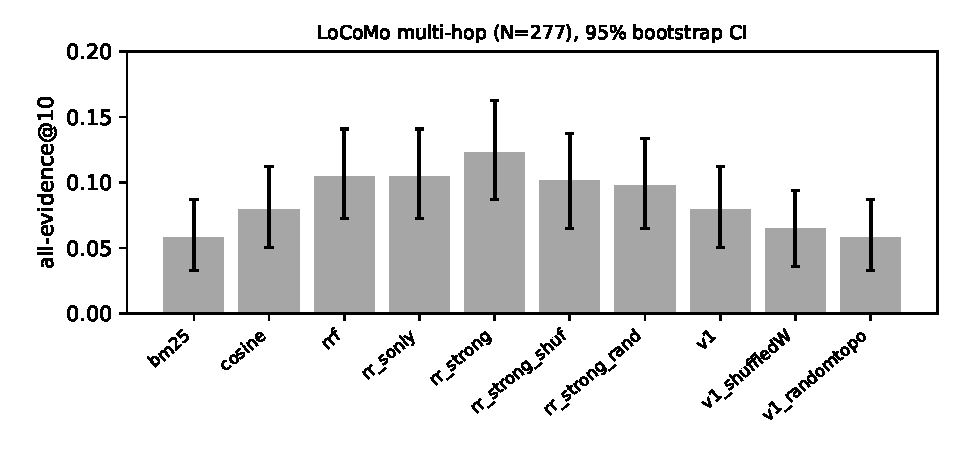
\includegraphics[width=0.49\linewidth]{figs/fig_retrieval.pdf}\hfill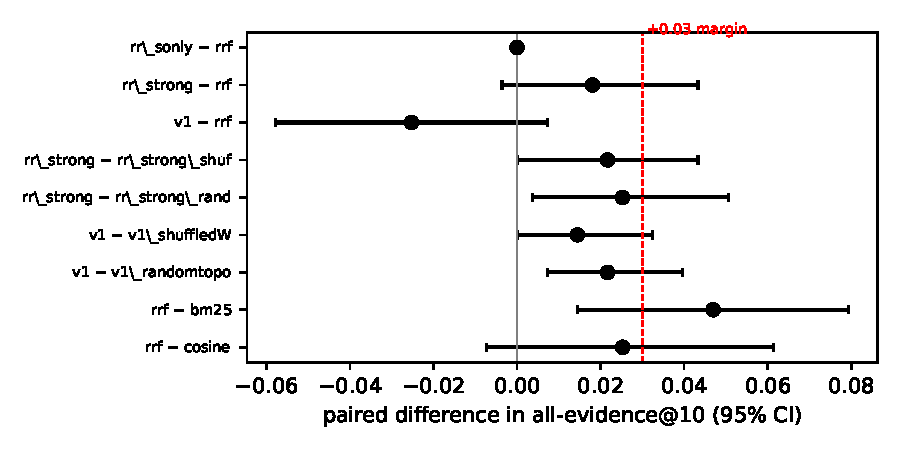
\includegraphics[width=0.49\linewidth]{figs/fig_paired.pdf}
\caption{Left: all-evidence@10 on the multi-hop population. Right: paired differences with 95\% CIs; dashed line is the pre-registered $+0.03$ margin.}\label{fig:ret}
\end{figure}

\begin{table}[h]
\centering\small
\begin{tabular}{lcc}\toprule
Paired difference (first $-$ second) & all-evidence@10 & evidence recall@10 (descriptive)\\\midrule
S-only: real vs shuffled $W$ & +0.000 [+0.000, +0.000] & +0.000 [+0.000, +0.000]  \\
S-only: real vs random edges & +0.000 [+0.000, +0.000] & +0.005 [+0.001, +0.011]  \\
Strong: real vs shuffled $W$ & +0.022 [+0.000, +0.043] & +0.024 [+0.004, +0.045]  \\
Strong: real vs random edges & +0.025 [+0.004, +0.051] & +0.025 [+0.005, +0.045]  \\
v1: real vs shuffled $W$ & +0.014 [+0.000, +0.032] & +0.026 [+0.005, +0.048]  \\
v1: real vs random topology & +0.022 [+0.007, +0.040] & +0.058 [+0.038, +0.078]  \\
v1: drop S & +0.004 [+0.000, +0.011] & +0.001 [-0.007, +0.010]  \\
v1: drop T & +0.011 [-0.011, +0.032] & +0.010 [-0.008, +0.029]  \\
v1: drop E & +0.000 [-0.011, +0.011] & -0.006 [-0.017, +0.004]  \\
v1: drop R (sanity: must be 0) & +0.000 [+0.000, +0.000] & +0.000 [+0.000, +0.000]  \\
v1: drop A* path & -0.007 [-0.018, +0.000] & -0.005 [-0.012, +0.001]  \\
Strong: drop S & +0.000 [+0.000, +0.000] & +0.004 [-0.004, +0.012]  \\
Strong: drop T & +0.000 [-0.018, +0.018] & -0.007 [-0.025, +0.011]  \\
Strong: drop E & -0.004 [-0.011, +0.000] & +0.001 [-0.008, +0.010]  \\
Strong: drop R (sanity) & +0.000 [+0.000, +0.000] & +0.000 [+0.000, +0.000] 
\\\bottomrule
\end{tabular}
\caption{Controls and ablations, multi-hop population ($N=277$), 95\% bootstrap CIs. ``Drop X'' rows are (ablated $-$ full). Dropping $R$ must give exactly zero without learning (sanity check; it does).}\label{tab:abl}
\end{table}

\textbf{Controls and ablations (Table~\ref{tab:abl}).} All S/T/E/A$^*$ ablations are within $\pm0.011$ on the primary metric and every CI contains zero or touches it at the boundary. Real topology beats random edges on the primary metric in point estimate ($+0.022$ [$+0.007,+0.040]$ for v1, raw $p=0.030$, Holm $0.57$). Real $W$ versus shuffled $W$: $0.000$ for S-only (the top-10 sets were identical in a 32-question spot check despite 5{,}192 differing entries of $W$), $+0.014$ for v1 and $+0.022$ for strong on the primary metric. On the graded recall metric the latter two are $+0.026$ and $+0.024$ with CIs above zero, but that is uncorrected, secondary, from one shuffle seed, and no single-factor ablation reproduces it. We treat it as a hint, not a finding. It has the opposite sign from LongMemEval-S, where shuffled weights did as well or better (nDCG@10 $+0.040$ for shuffled, with a retrieval-recall difference of $+0.006$ [$-0.015,0.028$]).

\subsection{End-to-end QA (R-2026-11-03-04)}
\begin{table}[h]
\centering\small
\begin{tabular}{lcc}\toprule
Arm & Partial-F1 [95\% CI] & All evidence in context\\\midrule
Z: closed-book (no context) & 0.145 [0.115, 0.178] & --  \\
A: RRF top-10 context & 0.258 [0.222, 0.296] & 0.105  \\
B: graph-bonus top-10 context & 0.258 [0.222, 0.295] & 0.105  \\
C: v1 retrieval, no draft & 0.220 [0.185, 0.257] & 0.079  \\
D: v1 retrieval + closed-book draft & 0.229 [0.194, 0.265] & -- 
\\\bottomrule
\end{tabular}\\[4pt]
\begin{tabular}{lccc}\toprule
Paired difference & Mean [95\% CI] & $p$ (raw) & $p_{\mathrm{Holm}}$\\\midrule
B $-$ A & -0.001 [-0.015, +0.013] & 0.936 & 0.94  \\
C $-$ A & -0.038 [-0.075, -0.003] & 0.036 & 0.11  \\
D $-$ C & +0.009 [-0.014, +0.032] & 0.446 & 0.89  \\
A $-$ Z & +0.113 [+0.075, +0.153] & $<$0.001 & -- 
\\\bottomrule
\end{tabular}
\caption{Qwen2.5-1.5B-Instruct on LoCoMo multi-hop ($N=277$). Holm over \{B$-$A, C$-$A, D$-$C\}; A$-$Z is a sanity check. Answers differ between A and B for 12 of 277 questions.}\label{tab:qa}
\end{table}
The primary label B$-$A is $-0.0006$ [$-0.015,+0.013$]; the falsifier fired. The context helps (A$-$Z $=+0.113$), but graph context equals fusion context because the contexts are nearly identical (B$-$A has low power by construction, which we stated in advance). Sandwich retrieval without the draft is $0.038$ below RRF context (Holm $p=0.11$). Contrary to the pre-registered prediction, adding the closed-book draft did not hurt ($+0.009$ [$-0.014,+0.032]$). Exploratory: D$-$A $=-0.029$ [$-0.067,+0.008]$. Predictions that held: A$-$Z $\ge+0.10$, B$-$A within $\pm0.02$, C$-$A $<0$ in point estimate, A's F1 in $[0.15,0.35]$. Predictions that failed in this run: D$-$C$<0$ (observed $+0.009$). Predictions that failed in the earlier runs: graph-as-first-stage $\le-0.05$ versus RRF in R-03 (observed $-0.025$), and RRF--cosine inside $[+0.02,+0.08]$ in R-02 (observed $+0.102$).

\section{Analysis}
\textbf{Draft contamination.} In an earlier synthetic run (v0; 120 probes; the primary model's window never contained the needed fact), feeding the primary draft to the secondary pass hurt: 94/120 correct versus 114/120 without the draft and 113/120 for plain RAG (exact McNemar versus RAG: 1 vs 20 discordant, $p<0.001$), concentrated in contradiction probes (19/40 vs 34/40), where the draft already agreed with the user's false claim. On LoCoMo with a 1.5B reader this effect is absent ($D-C=+0.009$). The synthetic task is saturated for retrieval (the gold value was in the top 4 for 120/120 probes for every retriever), so it tests anchoring, not memory. Our reading, not tested here, is that the anchoring cost depends on how often the draft is confidently wrong in a way the context could contradict; a 1.5B closed-book draft on LoCoMo is mostly just wrong or empty (F1 $0.145$).

\textbf{Weights carry no information.} Shuffling $W$ on the same edges, or dropping any of $S$, $T$ and $E$, does not change the primary metric beyond $\pm0.02$ in either dataset; on LongMemEval-S, removing $S$, $T$ or $E$ even raised nDCG. With $b=0$ and $R\equiv1$ the topology is a cosine $k$NN graph and $T$ and $E$ only re-weight edges that $S$ created. Without learning, $R$ cannot be tested at all (the $R$ ablation is an exact identity), and no experiment here trains $R$. The remaining honest statement is: the kNN topology is a (weak) signal; the weighting formula is untested for $R$ and unsupported for $S,T,E$.

\textbf{$\cn$ as an error signal.} On LongMemEval-S, AUROC of low $\cn$ for retrieval failure was $0.63$--$0.68$, below max-cosine ($0.72$--$0.74$) for failures of the cosine and graph retrievers, and slightly above it for BM25 failures ($0.625$ vs $0.603$); a residual analysis in the repository gave $0.56$--$0.59$. On the synthetic run, AUROC was $0.659$ ($n=120$, no CI). A refine-when-$\cn$-low trigger lost badly (44/120 vs 94/120 always refining), because $\cn$ is highest exactly when contradictory memories coexist. $\cn$ is mostly a restatement of retrieval confidence.

\textbf{Where the graph helps and where it does not.} It does not help as first stage (worse than or equal to cosine), as a conservative bonus (no change), or end-to-end with a small reader (no change). It may help slightly in the aggressive bonus configuration ($+0.018$, not significant), and kNN topology beats random edges by a small, mostly uncorrected margin on both datasets. The headroom is large: with the best retriever, all evidence is in the top 10 for only $10.5\%$ of multi-hop questions, and reader F1 is $0.565$ when all evidence is in context ($n=29$) versus $0.222$ when it is not ($n=248$; observational, not causal). The binding constraint is evidence recall for multi-evidence questions, which seeded activation from a weak first stage does not address.

\section{Limitations}
\textbf{Compute and models.} All runs are CPU-only; the encoder is MiniLM-L6 and the reader is a 1.5B model, greedy, one seed. Conclusions about weak encoders and small readers need not transfer to 7B+ models or stronger encoders; a larger reader could change both the draft effect and the ranking of arms. \textbf{No LLM judge.} QA is scored by lexical partial-F1, which rewards overlap and is noisy for free-form answers. \textbf{Power.} $N=277$ gives CIs of about $\pm0.03$ on all-evidence@10, so effects up to roughly $+0.04$ for the strong configuration are not excluded; B$-$A has low power by design. \textbf{Configuration transfer.} Settings were selected on LongMemEval-S, not LoCoMo; a re-tuned graph could do better. \textbf{Graph construction.} Only a MiniLM $k$NN graph was tested; no entity graph, no learned $R$, no conflict edges, no mood. \textbf{Labels and data.} LoCoMo evidence annotations contain malformed ids (4 questions affected) and are small (10 conversations); the LongMemEval-S development analyses were exploratory. Pre-registration is by git commit timestamp, not a public registry. \textbf{Single author.} No independent replication or code review.

\section{Conclusion}
A graph layer between two LLM calls is easy to specify precisely and hard to justify empirically. After auditing the specification into a bounded form, we tested it with pre-registered comparisons on two datasets. A fusion of BM25 and dense retrieval is the baseline to beat; the graph layer, as first stage, as conservative bonus, and end-to-end with a 1.5B reader, did not beat it. The weighting formula showed no measurable effect; topology gave at most a small one. Whether stronger encoders, entity-level graphs, learned reinforcement, or larger readers would change this is open, and the protocol and code allow testing it cheaply.

\section*{Reproducibility Statement}
Everything is in one repository (public URL \todo{add after the repository is published}): \texttt{src/conslayer/} (\texttt{theory\_v1.py}, \texttt{stats.py}, \texttt{runlog.py}, \texttt{locomo\_eval.py}), \texttt{experiments/} (one script per run), \texttt{tests/} (52 passing unit tests), \texttt{docs/} (\texttt{THEORY\_V1.md}, \texttt{MATH\_AUDIT.md}, \texttt{THEORY\_LEDGER.md}, \texttt{STATUS.md}), \texttt{LAB\_NOTEBOOK.md} (pre-registrations, results, surprises, aborted runs), \texttt{results/<run\_id>/} (config with commit hash and package versions, per-question CSVs) and \texttt{paper/} (this paper; \texttt{make\_figs.py} generates every table and figure from the result CSVs). Runs: R-2026-11-03-01 (embedding cache, 13~s), -02, -03 (77~s), -04 (12.9~min) on 8 CPU cores. Models: all-MiniLM-L6-v2, Qwen2.5-1.5B-Instruct. LoCoMo is CC BY-NC 4.0; we do not redistribute it. A claim ledger tracks 43 claims with their status (6 supported, 19 refuted, 5 mixed, 3 weak, 3 untested, 7 not testable).

\bibliographystyle{plain}
\bibliography{refs}
\end{document}
